\documentclass[11pt,a4paper]{article}
\usepackage[utf8]{inputenc}
\usepackage[greek,english]{babel}
\usepackage{alphabeta}
\usepackage{amsmath}
\usepackage{graphicx}
\usepackage{hyperref}
\usepackage{listings}
\usepackage{caption}
\usepackage{geometry}
\geometry{a4paper, margin=1in}

\lstset{
    basicstyle=\ttfamily\footnotesize,
    breaklines=true,
    frame=single,
    showstringspaces=false,
    captionpos=b
}

\title{
  \vspace{-2cm}
  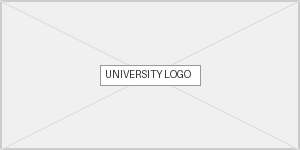
\includegraphics[width=1.8cm]{university_logo_placeholder.png}\\[0.5cm]
  \textbf{Επεξεργασία Δεδομένων Ροής με Kafka, Spark και MongoDB}\\
  \large Συστήματα Διαχείρισης Μεγάλων Δεδομένων (CEID\_NE4348)
}
\author{
  Βερύκιος Άγγελος (Α.Μ: 1100500) \\
  Βογιαντζής Αναστάσιος (Α.Μ: 1100506)
}
\date{Ιούνιος 2026}

\begin{document}

\maketitle

\section{Εισαγωγή και Σκοπός της Εργασίας}
Η εκθετική αύξηση των δεδομένων που παράγονται καθημερινά, ειδικά στο πλαίσιο του Internet of Things (IoT) και των έξυπνων πόλεων (Smart Cities), επιτάσσει την ανάγκη για συστήματα που μπορούν να επεξεργάζονται την πληροφορία σε πραγματικό χρόνο (real-time stream processing). Σκοπός της παρούσας εργασίας είναι η σχεδίαση και υλοποίηση μιας ολοκληρωμένης, επεκτάσιμης εφαρμογής ανάλυσης ροής δεδομένων, η οποία λειτουργεί ως data streaming pipeline. 

Η εφαρμογή προσομοιώνει την κίνηση οχημάτων σε ένα πολύπλοκο οδικό δίκτυο με διασταυρώσεις και φανάρια. Τα δεδομένα που παράγονται (ταχύτητες, συντεταγμένες, χρόνος) συλλέγονται άμεσα μέσω ενός message broker. Στη συνέχεια, ένα κατανεμημένο υπολογιστικό σύστημα τα αναλύει για την εξαγωγή κρίσιμων στατιστικών, όπως το πλήθος οχημάτων και η μέση/μέγιστη ταχύτητα ανά τμήμα δικτύου (link). Τέλος, το pipeline καταλήγει σε μια NoSQL βάση δεδομένων για μόνιμη αποθήκευση, παρέχοντας ταυτόχρονα διεπαφές για την ανάγνωσή τους.

\section{Περιγραφή Αρχιτεκτονικής Συστήματος}
Το σύστημα υλοποιήθηκε ακολουθώντας τις αρχές των μικροϋπηρεσιών (microservices architecture). Η προσέγγιση αυτή εξασφαλίζει ότι το κάθε υποσύστημα λειτουργεί ανεξάρτητα. Για την ενορχήστρωση χρησιμοποιήθηκε το \textbf{Docker Compose}, επιτρέποντας την ταυτόχρονη και δικτυωμένη εκκίνηση των παρακάτω υπηρεσιών:

\begin{itemize}
    \item \textbf{Data Producer (Python \& UXSIM):} Το αυτόνομο περιβάλλον προσομοίωσης που δημιουργεί τον όγκο των δεδομένων. Λειτουργεί ως αφετηρία του pipeline και παράγει χιλιάδες εγγραφές ανά λεπτό.
    \item \textbf{Message Broker (Redpanda):} Μια σύγχρονη, υψηλών επιδόσεων υπηρεσία, πλήρως συμβατή με το Kafka API. Είναι υπεύθυνη για την ασφαλή προσωρινή αποθήκευση των δεδομένων στο topic \texttt{vehicle\_positions}, αντέχοντας τεράστιο φόρτο.
    \item \textbf{Stream Processing Engine (Apache Spark):} Ο πυρήνας επεξεργασίας του συστήματος, ενορχηστρωμένος σε Master-Worker topology. Το PySpark καταναλώνει τα δεδομένα ως συνεχές ρεύμα (Structured Streaming) και εφαρμόζει τους μετασχηματισμούς.
    \item \textbf{NoSQL Storage (MongoDB):} Ως βάση δεδομένων εγγράφων, η MongoDB προσφέρει την απαραίτητη ευελιξία για να αποθηκεύσει το παραγόμενο JSON χωρίς άκαμπτα σχήματα (schemas).
    \item \textbf{RESTful API (Flask - Bonus):} Ένα επιπλέον microservice που γεφυρώνει τη MongoDB με τον τελικό χρήστη, διαθέτοντας τα στατιστικά μέσω HTTP αιτημάτων.
\end{itemize}

\section{Σχεδιαστικές Επιλογές και Υλοποίηση}

\subsection{Παραγωγή Δεδομένων και Διαχείριση Ροής}
Η παραγωγή των δεδομένων (\texttt{producer.py}) απαιτούσε προσοχή ώστε να μην "πνιγεί" το δίκτυο με περιττή πληροφορία. Η αρχική προσομοίωση παράγει στιγμιότυπα (snapshots) για κάθε χρονικό βήμα. Ως σχεδιαστική επιλογή, αποφασίστηκε να εφαρμόζεται \textbf{φιλτράρισμα} σε επίπεδο παραγωγού: αποστέλλονται μόνο τα οχήματα που βρίσκονται σε κίνηση (δηλαδή με ταχύτητα \texttt{speed > 0}). Αυτό μειώνει δραματικά τον όγκο των δεδομένων. 

Η αποστολή γίνεται μετατρέποντας το Python Dictionary σε JSON (serialization) και στέλνοντάς το μέσω της βιβλιοθήκης \texttt{kafka-python}. Επιπλέον, προστέθηκε δυνατότητα παραμετροποίησης του χρόνου (interval) μέσω ορισμάτων γραμμής εντολών (\texttt{argparse}), καθώς και μηχανισμοί χειρισμού σφαλμάτων (try-except) για ομαλή επανασύνδεση.

\subsection{Structured Streaming και Aggregations στο Spark}
Το στάδιο της κατανάλωσης (\texttt{spark\_consumer\_PC.py}) ήταν το πιο απαιτητικό. Η εφαρμογή διαβάζει τα binary δεδομένα από το Redpanda και τα κάνει cast σε string για να διαβαστούν ως JSON βάσει του \texttt{StructType} που ορίστηκε. 

Πέρα από τις βασικές μετρικές (υπολογισμός \texttt{vcount} και μέσης ταχύτητας \texttt{vspeed}), η ομάδα μας υλοποίησε \textbf{όλα τα προαιρετικά (Bonus) ερωτήματα}:
\begin{enumerate}
    \item \textbf{Ενισχυμένα Στατιστικά:} Προστέθηκαν μετρικές για τον υπολογισμό της μέγιστης (\texttt{vmax}) και ελάχιστης (\texttt{vmin}) ταχύτητας ανά ακμή δικτύου.
    \item \textbf{Windowed Aggregations (Χρονικά Παράθυρα):} Δημιουργήθηκε ένα επιπλέον επίπεδο aggregations (buckets), όπου τα δεδομένα ομαδοποιούνται ανά 30 δευτερόλεπτα. Αυτό επιτρέπει την παρακολούθηση της κίνησης σε βάθος χρόνου (trend analysis) αντί για απόλυτες στιγμιαίες τιμές.
\end{enumerate}

\subsection{Στρατηγική Αποθήκευσης στη MongoDB}
Για την εγγραφή χρησιμοποιείται η μέθοδος \texttt{foreachBatch}. Η επιλογή αυτή προσφέρει τον απόλυτο έλεγχο πάνω στο πώς κάθε micro-batch εγγράφεται στη βάση. Δημιουργήθηκε μια generic βοηθητική συνάρτηση (\texttt{make\_mongo\_writer}) η οποία επαναχρησιμοποιείται για να κατευθύνει τα δεδομένα:
Τα αρχικά JSON μηνύματα σώζονται στη συλλογή \texttt{raw\_data} (με \texttt{append} mode), ενώ τα στατιστικά στις \texttt{stats} και \texttt{windowed\_stats} (με \texttt{update} mode).

\section{Προβλήματα που Αντιμετωπίστηκαν και Λύσεις}
Κατά τη διάρκεια ανάπτυξης της υποδομής, προέκυψαν οι εξής τεχνικές προκλήσεις:
\begin{enumerate}
    \item \textbf{Race Conditions στην Εκκίνηση:} Το PySpark job συχνά αποτύγχανε αν το Redpanda ή η MongoDB δεν είχαν προλάβει να ξεκινήσουν τις θύρες επικοινωνίας τους. Αυτό λύθηκε προσθέτοντας τα κατάλληλα \texttt{depends\_on} στο αρχείο \texttt{docker-compose.yml} και μηχανισμούς retries στους κώδικες της Python.
    \item \textbf{Εξαρτήσεις του PySpark (JAR Hell):} Η ενσωμάτωση του Kafka και της MongoDB απαιτούσε τη φόρτωση εξωτερικών βιβλιοθηκών Java. Η απουσία έστω και ενός (π.χ. \texttt{bson.jar} ή \texttt{commons-pool2.jar}) οδηγούσε σε \texttt{ClassNotFoundException}. Η λύση ήταν ο αυστηρός καθορισμός όλων των dependencies στο όρισμα \texttt{--jars} κατά την υποβολή του \texttt{spark-submit}.
    \item \textbf{Τύποι Δεδομένων (NumPy to JSON):} Η βιβλιοθήκη UXSIM χρησιμοποιεί τύπους όπως \texttt{numpy.float64}. Η εγγενής βιβλιοθήκη JSON της Python αδυνατεί να τους κάνει serialize, προκαλώντας crash στον παραγωγό. Λύθηκε αναπτύσσοντας τη συνάρτηση \texttt{convert()} που σαρώνει και μετατρέπει δυναμικά τα δεδομένα σε native τύπους (int, float).
\end{enumerate}

\section{Αναλυτική Παρουσίαση και Στιγμιότυπα Εκτέλεσης}
Στην παρούσα ενότητα παρουσιάζεται η πραγματική ροή εκτέλεσης της εφαρμογής μέσα από μια σειρά σεναρίων ελέγχου, αποδεικνύοντας τη διαλειτουργικότητα των συστημάτων.

\subsection{Προσομοίωση και Αποστολή Δεδομένων}
Η διαδικασία ξεκινά με την εκκίνηση του UXSIM. Ο κώδικας αρχικοποιεί το δίκτυο, υπολογίζει τις συντεταγμένες και αρχίζει να παράγει εγγραφές ανά τακτά χρονικά διαστήματα (Σχήμα 1). Καθώς τα δεδομένα παράγονται, ταξιδεύουν μέσω του τοπικού δικτύου του Docker προς το topic \texttt{vehicle\_positions} του Redpanda broker, περιμένοντας να καταναλωθούν (Σχήμα 2).

\begin{center}
    
\includegraphics[width=0.95\textwidth]{producer_output.png} 
    \captionof{figure}{Εκτέλεση του παραγωγού και αποστολή μηνυμάτων.}
    
    \vspace{0.4cm} % Μικρό κενό ανάμεσα στις εικόνες
    
    
\includegraphics[width=0.95\textwidth]{redpanda_topic.png} 
    \captionof{figure}{Λήψη των JSON μηνυμάτων από το Broker.}
\end{center}


\subsection{Επεξεργασία Ροής και Υπολογισμός (Spark)}

\begin{minipage}[t]{0.56\textwidth}
  \vspace{0pt}
  Η πιο κρίσιμη διεργασία λαμβάνει χώρα εντός του Apache Spark. Όπως παρατηρούμε στο Σχήμα 3, το Spark Structured Streaming χωρίζει τη συνεχή ροή σε διακριτά "Batches" (micro-batches) με προκαθορισμένο trigger interval. 
  
  \medskip
  Στον πίνακα της κονσόλας φαίνονται ξεκάχαρα οι στήλες που έχουμε ορίσει: ο χρόνος προσομοίωσης (\texttt{time}), το τμήμα του δικτύου (\texttt{link}) και οι βασικές μετρικές, δηλαδή το πλήθος των οχημάτων (\texttt{vcount}) και η μέση ταχύτητά τους (\texttt{vspeed}).

  \medskip
  Επιπλέον, αποδεικνύεται η ορθή λειτουργία των \textbf{Bonus ερωτημάτων}, καθώς στον πίνακα έχουν προστεθεί και τυπώνονται ζωντανά οι τιμές μέγιστης (\texttt{vmax}) και ελάχιστης (\texttt{vmin}) ταχύτητας.

  \medskip
  Αμέσως κάτω από τους πίνακες, το Spark επιβεβαιώνει την επικοινωνία του με τη βάση δεδομένων εκτυπώνοντας τα μηνύματα \texttt{MongoDB OK} για κάθε ξεχωριστό batch. Σημειώνεται ότι εκτός από τα \texttt{[stats]} και \texttt{[raw\_data]}, το σύστημα αποθηκεύει επιτυχώς και τα \texttt{[windowed\_stats]}, τα οποία αφορούν τον υπολογισμό των κινητών μέσων όρων ανά 30 δευτερόλεπτα (το δεύτερο Bonus).

  \medskip
  Η λειτουργία του Spark Streaming παραμένει ενεργή και αδιάλειπτη καθ'όλη τη διάρκεια της προσομοίωσης, χωρίς να παρατηρούνται καθυστερήσεις (bottlenecks) στη μνήμη του Worker node.
\end{minipage}
\hfill
\begin{minipage}[t]{0.39\textwidth}
  \vspace{0pt} 
  \centering
  
\includegraphics[width=\textwidth]{spark_console_bonus.png}
  \captionof{figure}{Έξοδος του Spark Console που απεικονίζει τα micro-batches.}
\end{minipage}
\vspace{0.5cm}

\subsection{Μόνιμη Αποθήκευση στη MongoDB}
Η τρίτη φάση του pipeline αφορά την επικύρωση των εγγραφών στη βάση δεδομένων. Μέσω του κελύφους \texttt{mongosh}, πραγματοποιήθηκαν ερωτήματα επιβεβαίωσης. Στο Σχήμα 4, παρουσιάζεται η εντολή \texttt{findOne()} τόσο για τη συλλογή \texttt{raw\_data} (όπου βλέπουμε την ακατέργαστη εγγραφή ενός οχήματος) όσο και για τη συλλογή \texttt{stats} (όπου βλέπουμε το aggregated document).

Προκειμένου να αποδειχθεί η δυνατότητα άντλησης σύνθετων πληροφοριών μετά την ολοκλήρωση του pipeline, γράφτηκε ένα Aggregation Query, το οποίο διατρέχει όλη τη συλλογή \texttt{stats} και υπολογίζει τον συνολικό μέσο όρο ταχύτητας ανά \texttt{link}:
\begin{verbatim}
db.stats.aggregate([ 
  { $group: { _id: "$link", avg_overall_speed: { $avg: "$vspeed" } } } 
])
\end{verbatim}
Τα αποτελέσματα του παραπάνω ερωτήματος αποτυπώνονται στο Σχήμα 5.

\begin{center}
    
\includegraphics[width=0.75\textwidth]{mongo_collections.png} 
    \captionof{figure}{Ανάκτηση εγγραφών (raw και aggregated) από τη MongoDB.}
    
    \vspace{0.4cm}
    
    
\includegraphics[width=0.75\textwidth]{aggregation.png} 
    \captionof{figure}{Εκτέλεση του Aggregation Query για την εξαγωγή του συνολικού μέσου όρου.}
\end{center}

\subsection{Διεπαφή Χρήστη (REST API - Bonus)}
Τέλος, το API που κατασκευάστηκε σε Flask εκτελείται στην πόρτα 5000. Στο Σχήμα 6 φαίνεται η εκκίνηση του server. 

\begin{center}
    
\includegraphics[width=0.8\textwidth]{rest_api.png} 
    \captionof{figure}{Εκκίνηση του REST API Server.}
\end{center}

Μέσω αυτού του API, οποιοσδήποτε client (π.χ. ένα Dashboard) μπορεί να αντλήσει τα δεδομένα. Παρακάτω παρατίθεται η απόκριση (JSON Response) του συστήματος από το endpoint \texttt{/api/windowed}, το οποίο επιβεβαιώνει τον υπολογισμό των Windowed Aggregations:

\begin{lstlisting}[caption=Πραγματική απόκριση του REST API για το /api/windowed]
{
  "window_start": 120.0,
  "link": "E1I4",
  "vcount": 13,
  "avg_speed": 40.76,
  "max_speed": 50.00,
  "min_speed": 20.00
}
\end{lstlisting}

Συμπερασματικά, μέσω της πλήρους εκτέλεσης της υποδομής, αποδεικνύεται η αδιάληπτη λειτουργία ενός ολοκληρωμένου, fault-tolerant Big Data Pipeline, το οποίο καλύπτει επιτυχώς όλες τις απαιτήσεις της εργασίας.

\end{document}
